\section{Co-training Framework}
	\label{sec:Co-Train}
	\begin{figure}
	\centering 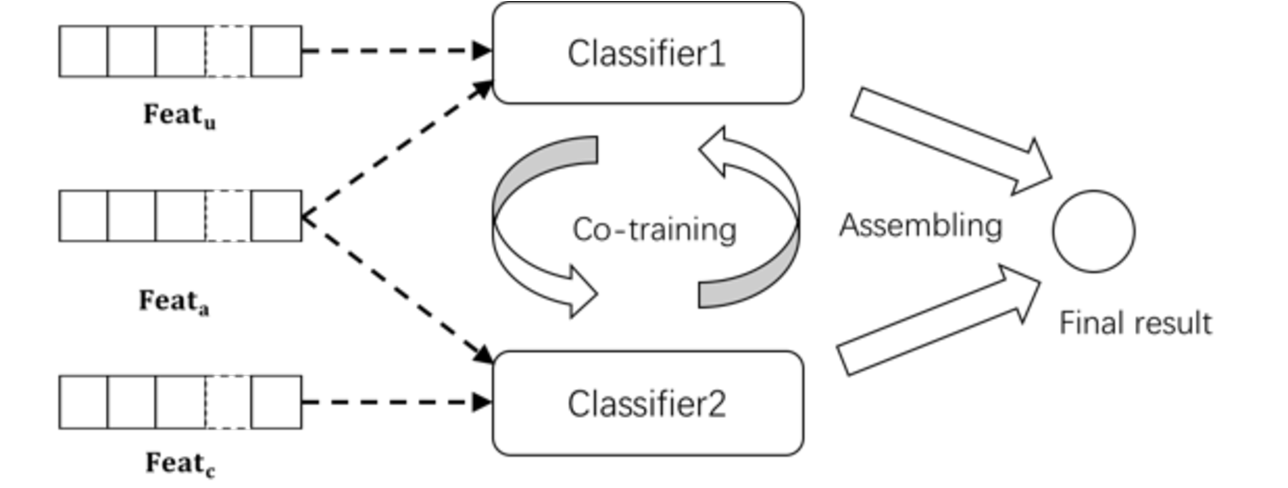
\includegraphics[width=9cm]{architecture.pdf}
	\caption{The Illustration of Dropout Prediction Framework.}
	\label{fig:arch}
	\end{figure}
	In order to combine features extracted from different sources, we design a multiview based Co-training framework. There are two classifiers in this framework. One is used to learn user individual preference, while the other one is to learn course-related preference.  Moreover, the Co-training framework can leverage unlabeled data to facilitate the prediction performance on the sparse personalized data. Specifically, Co-training framework consists of three steps.
	\begin{itemize}
		\item {\textbf{Constructing multiple classifiers.}} The first step is to construct multiple classifiers with good diversity based on the three types of features: $\mathbf{Feat}_a$, $\mathbf{Feat}_u$ and $\mathbf{Feat}_c$.
		
		\item{\textbf{Co-Training.}} In the Co-Training procedure, each classifier can learn from each other. More accurately, those examples with high confidences are selected for the classifier and being labeled based on the predict probability score,  and then they are used to ``teach" the other classifier.
		\item{\textbf{Assembling the results.}} In the end, the probability scores obtained by individual classifiers are assembled to the final prediction score.
	\end{itemize}
	Algorithm \ref{alg:Co-Training} gives the details of the Co-training algorithm, and the whole architecture of our dropout prediction framework is illustrated in Figure \ref{fig:arch}.
	\begin{algorithm}[!h]
		\caption{Co-Training Algorithm.}  
		\label{alg:Co-Training}  
		\KwIn{the training set $L$, and the test example set $U$;}
		\KwOut{classifier $h(u,c)$ for dropout prediction;}
		\textbf{Step 1: Construct Multiple classifiers}\\
		Generate two classifiers $h_1$ and $h_2$ based on multiviews;\\
		Initialize the training sets of $h_1$ and $h_2$: $L_1=L $, $L_2 = L$; \\  
		Create a pool $U'$ by randomly picking $\mathcal{U}$ examples from $U$;\\
		\textbf{Step 2: Co-Training}\\
		\Repeat{$\mathcal{T}$ rounds}{
			\For {j=1 to 2}{
				Training $h_j$ on the corresponding training set $L_1$ and labeling the examples in $U'$;\\
				Constructing teaching set $T_j$ by selecting $p$ positive and $n$ negative examples from $U'$;\\
				$U' = U'-T_j$;
			}
		    Randomly choose $2p+2n$ examples from $U$ to replenish $U'$\\
			Teach peer classifiers: $L_1=L_1 \cup T_2$; $L_2=L_2 \cup T_1$;\\
			%Update the two classifiers: $h_1\leftarrow L_1$; $h_2\leftarrow L_2$;
		}
		\textbf{Step 3: Assembling the results} $h(u,c)=Assemble(h_1(u,c), h_2(u,c))$
	\end{algorithm}

	
	\subsection{Constructing multiple classifiers}
	\label{sec:construct}
	Generating multiple classifiers with good diversity is the key point in the Co-training framework. Here we employ a multiview based method to construct different classifiers. Multiview mechanism has been widely used in many different machine learning topics. Here we adopt this method to construct different classifiers. In this method, all features (described in Section \ref{sec:allFeat})  are divided into two sets: $\{\mathbf{Feat}_a, \mathbf{Feat}_u\}$ and $\{\mathbf{Feat}_a, \mathbf{Feat}_c\}$. Then the two sets of features are input to two different classifiers, respectively. We denote the two classifiers as $h_1$ and $h_2$, and they can be formalized as follows.
	\begin{equation}
	h_1(u,c) = g([\mathbf{Feat}_{a}, \mathbf{Feat}_{u}])\end{equation}
	\begin{equation}h_2(u,c)=g([\mathbf{Feat}_{a}, \mathbf{Feat}_{c}])
	\end{equation}
	Where $g(\cdot)$ is the classify function. $h_1$ is used to capture individual preference from the perspective of user, while $h_2$ is learning course-related preference information. Based on previous work\cite{Zhou:2005:SRC:1642293.1642439}, each learner of the Co-training framework should be sufficient for each learner in the Co-training framework to learn. In order to meet the requirement, Activity Features $\mathbf{Feat}_a$ are input to both classifiers as the extra feature set. 
	
	\subsection{Semi-supervised Co-training}
	\label{sec:co-training}
		After constructing multiple classifiers, the task amounts to co-training the different classifiers. For each classifier $j$, we need to construct a ``teaching set" $T_j$ from the unlabeled samples and use it to teach the other classifier. Before that, we must label the unlabeled examples based on the classification confidences produced by each classifier. Moreover, In order to make this procedure more efficient, a smaller pool set $U'$ is drawn randomly from the whole unlabeled set $U$ before co-training. This was proved to be helpful for improving the final performance in the previous work\cite{Blum:1998:CLU:279943.279962}.\\
	
	\noindent \textbf{Labeling the unlabeled examples}
    
	Labeling is the final step for most of the classifier systems, in which the unlabeled samples are labeled based on their classification scores. For binary classification, a general labeling strategy is to compare classification score with a decision threshold $\gamma$. If the score of an example is higher than $\gamma$, then the example is set to positive, otherwise, it is set to negative. $\gamma$ is usually set to $0.5$ when the classification score is from $0$ to $1$.  However, this strategy does not work on the imbalanced datasets of dropout prediction task. To alleviate the imbalanced classification problem, we propose a ranking based labeling strategy with three steps:
	\begin{itemize}
		\item Calculate the ratio $r$ of positive examples to all examples in training set: $r=\frac{|P_L|}{|N_L|+|P_L|}$, where $P_L$ is the set of positive examples and $N_L$ is the set of negative examples.
		\item Rank all the examples in $U'$ using their classification score.
		\item Label top $r * |U'|$ examples in $U'$ as positive, and others as negative.
	\end{itemize}
    Next, the classification confidence of example $x_{uc}$ predicted by classifier $j$ is:
    \begin{equation}
    C_j(x_{uc})=l_{x_{uc}}*s_{x_{uc}} + (1-l_{x_{uc}})*(1-s_{x_{uc}})
    \end{equation}
    where $s_{x_{uc}}$ is the classification score of $x_{uc}$, and $l_{x_{uc}} \in \{0,1\}$ is its corresponding label. $l_{x_{uc}} = 1$ means $x_{uc}$ is positive, while $l_{x_{uc}} = 0$ indicates that the example is negative. As shown above, if $x_{uc}$ is labeled to positive, the corresponding confidence is  its classification score $s_{x_{uc}}$, and if $x_{uc}$ is negative, its confidence is $1- s_{x_{uc}}$.\\
    
    
    \noindent \textbf{Constructing Teaching Set and Co-training}
    
    For constructing the ``teaching set'' $T_j$ for each classifier $j$, we adopt Roulette algorithm \cite{Back:1996:EAT:229867} to sample examples randomly from $U'$ based on their confidences. The sample probability of each example is calculated by:
     \begin{equation}
     Pr(x_{uc}, j)=\frac{C_j(x_{uc})}{\sum_{x_i\in U'}C_j(x_i)}
     \end{equation}
     We sample $p$ positive examples and $n$ negative examples to construct $T_j$ for each classifier $j$.
    After selecting examples from $U'$, we need to choose $2p+2n$ examples from test set $U$ to replenish $U'$. Finally the examples in one teaching set $T_j$ are merged into the training set of the other classifier. In this way, the unlabeled data are incorporated into the learning process. This procedure of constructing the teaching sets and Co-training will be repeated for $\mathcal{T}$  iterations in this algorithm.
    \subsection{Assembling the Results}
    \label{sec:assemble}
    The results of two classifiers are assembled together in the final step. A general method is to compute the mean value for all the classification scores, i.e.,
    \begin{equation}
    h(u,c) =\frac{1}{l}\sum_{j=1...l}h_j(u, c)
    \end{equation}
    
    where $l$ is the number of classifiers being assembled. In our case, the ensemble scheme for two classifiers is $h(u,c) = \frac{1}{2}[h_1(u,c)+h_2(u,c)]$. However, this method does not consider the classification confidence of different classifiers. To address this problem, we assemble the results by taking weighted average of all results. Here the weights are computed by the classification confidences, i.e.,
    \begin{equation}
    h(u,c)=\sum_{j=1...l}\frac{C_j(x_{uc})}{\sum_{k=1...l}C_k(x_{uc})}h_j(u,c)
    \end{equation}
    Another option for computing weights is based on the average AUC score of k-fold cross validation: $h(u,c)=\sum_{j=1...l}\frac{w_j}{\sum_{k=1...l}w_k}h_j(u,c)$. Where $w_j$ is the average AUC score of the $h_j$'s k-fold cross validation on training set. However, running k-fold cross validation means that the model must be trained $k$ times on training set, which is less efficient in practice. 
    Note that these ensemble methods can either be applied right after the training of individual models without the Co-training. By this way, the framework only makes use of the labeled data, while the Co-training framework can consider not only labeled data but also unlabeled data.